\chapter*{Dodatak: Prikaz aktivnosti grupe}
		\addcontentsline{toc}{chapter}{Dodatak: Prikaz aktivnosti grupe}
		
		\section*{Dnevnik sastajanja}
		
		\begin{packed_enum}
			\item  sastanak
			
			\item[] \begin{packed_item}
				\item Datum: 19. listopada 2023.
				\item Prisustvovali: L. Topolko, J. Kolarec, I.Svalina, I. Kvesić, N. Lazarić, F. Mišković, B. Marković
				\item Teme sastanka:
				\begin{packed_item}
					\item dogovor o korištenim tehnologijama
					\item dogovor o načinima komunikacije
					\item podjela u timove za frontend, backend i dokumentaciju
					\item definiranje osnovnih funkcionalnosti
				\end{packed_item}
			\end{packed_item}
			
			\item  sastanak
			\item[] \begin{packed_item}
				\item Datum: 23. listopada 2023.
				\item Prisustvovali: L. Topolko, J. Kolarec, I.Svalina, I. Kvesić, N. Lazarić, F. Mišković, B. Marković
				\item Teme sastanka:
				\begin{packed_item}
					\item sastavljanje use-caseova
					\item razgovor o povezivanju frontenda i backenda
					\item dogovor o bazi i sadržaju baze
				\end{packed_item}
			\end{packed_item}
			
			\item  sastanak
			\item[] \begin{packed_item}
				\item Datum: 24. listopada 2023.
				\item Prisustvovali: L. Topolko, N. Lazarić, I. Svalina
				\item Teme sastanka:
				\begin{packed_item}
					\item  osmišljavanje baze podataka (odabir h2 baze za lokalno testiranje, odabir entiteta i njihovih atributa)
				\end{packed_item}
			\end{packed_item}
			
			\item  sastanak
			\item[] \begin{packed_item}
				\item Datum: 26. listopada 2023.
				\item Prisustvovali: F. Mišković, I. Kvesić, B. Marković
				\item Teme sastanka:
				\begin{packed_item}
					\item  dogovor o podjeli posla
					\item  određen okvirni izgled stranice
				\end{packed_item}
			\end{packed_item}
		
		
			\item  sastanak
			\item[] \begin{packed_item}
				\item Datum: 9. studenoga 2023.
				\item Prisustvovali: L. Topolko, J. Kolarec, I. Kvesić, N. Lazarić, F. Mišković, B. Marković
				\item Teme sastanka:
				\begin{packed_item}
					\item  od nastavnice dobivena povratna informacija o dosadašnjem radu 
					\item  utvrđivanje zadataka koje je potrebno dovršiti do prve predaje 
					\item dogovor o budućem izgledu pojedinih stranica web aplikacije
				\end{packed_item}
			\end{packed_item}
			
			
			\item  sastanak
			\item[] \begin{packed_item}
				\item Datum: 7. prosinca 2023.
				\item Prisustvovali: L. Topolko, J. Kolarec, I. Kvesić, N. Lazarić, B. Marković
				\item Teme sastanka:
				\begin{packed_item}
					\item dodjela bodova ostvarenih prilikom prve predaje projekta
				\end{packed_item}
			\end{packed_item}
			
			
			
			\item  sastanak
			\item[] \begin{packed_item}
				\item Datum: 11. siječnja 2024.
				\item Prisustvovali: L. Topolko, J. Kolarec, I. Svalina, I. Kvesić, N. Lazarić, F. Mišković, B. Marković
				\item Teme sastanka:
				\begin{packed_item}
					\item kontrolna točka prije konačne predaje projekta
					\item uputa i dogovor o daljnjem radu do predaje 
				\end{packed_item}
			\end{packed_item}
			
			
			\item  sastanak
			\item[] \begin{packed_item}
				\item Datum: 16. siječnja 2024.
				\item Prisustvovali: L. Topolko, J. Kolarec, I. Svalina, I. Kvesić, N. Lazarić, F. Mišković, B. Marković
				\item Teme sastanka:
				\begin{packed_item}
					\item podjela zadataka vezanih za prezentaciju projekta
					\item prezentacija i objašnjavanje vlastitih zadataka pojedinog člana tima ostalim članovima 
				\end{packed_item}
			\end{packed_item}
			
		
		
		\end{packed_enum}
		
		
		
		\eject
		\section*{Tablica aktivnosti}
		
			\vspace{-0.1cm}
			
			U tablici su navedeni doprinosi članova grupe u satima po pojedinoj aktivnosti. 
		
			\begin{longtblr}[
					label=none,
				]{
					vlines,hlines,
					width = \textwidth,
					colspec={X[7, l]X[1, c]X[1, c]X[1, c]X[1, c]X[1, c]X[1, c]X[1, c]}, 
					vline{1} = {1}{text=\clap{}},
					hline{1} = {1}{text=\clap{}},
					rowhead = 1,
				} 
			
				\SetCell[c=1]{c}{} & \SetCell[c=1]{c}{\rotatebox{90}{\textbf{Lucija Topolko}}} & \SetCell[c=1]{c}{\rotatebox{90}{\textbf{Natali Lazarić}}} &	\SetCell[c=1]{c}{\rotatebox{90}{\textbf{Julijana Kolarec }}} & \SetCell[c=1]{c}{\rotatebox{90}{\textbf{Iva Kvesić }}} &	\SetCell[c=1]{c}{\rotatebox{90}{\textbf{Bruno Marković}}} & \SetCell[c=1]{c}{\rotatebox{90}{\textbf{Filip Mišković}}} &	\SetCell[c=1]{c}{\rotatebox{90}{\textbf{Iva Svalina}}} \\  
				Upravljanje projektom 		& 7 &  &  &  &  &  & \\
				Sastanci  					& 6 & 6 & 6 & 6 & 6 & 6 & 6 \\ 
				Opis projektnog zadatka 	& 3 &  &  &  &  &  & \\ 
				
				Funkcionalni zahtjevi       & 1 &  & 2 &  &  &  &  \\ 
				Opis pojedinih obrazaca 	&  &  & 8 &  &  &  &  \\ 
				Dijagram obrazaca 			&  &  & 3 &  &  &  &  \\ 
				Sekvencijski dijagrami 		&  &  & 3 &  &  &  &  \\ 
				Opis ostalih zahtjeva 		&  &  & 1 &  &  &  &  \\ 

				Arhitektura i dizajn sustava	 &  &  & 2 &  &  &  &  \\ 
				Baza podataka				&  &  & 3 &  &  &  &   2\\ 
				Dijagram razreda 			& 2 &  & 7 &  &  &  &   \\ 
				Dodatak	 		 			&  &  & 1 &  &  &  &   \\
				Pravopis, čitljivost, opći dojam &  &  & 2 &  &  &  &   \\ 
				Backend & 10 & 12 &  &  &  &  &   \\ 
				Security  & 2 &  &  &  &  &  & 8 \\ 
				Deployment  & 20 & 22 &  &  &  &  & 15\\ 
				Istraživanje  & 2 & 1 &  1 & 8 & 8 & 8 & 10 \\ 
				Izrada baze podataka  & 2 &  &  &  &  &  & 3 \\ 
				Spajanje s bazom podataka
				 & 3 &  &  & 7 & 3 & 8  & 1  \\ 
				Izrada početne stranice  &  &  &  & 5 & 1 & 1 &   \\ 
				Izrada navigacijske trake  &  &  &  & 10 &  & 2 &   \\ 
				Izrada stranice za prijavu  &  &  &  &  & 13 & 2 &   \\ 
				\textbf{Ukupno do 1. revizije:} & \textbf{58} & \textbf{41}  & \textbf{39} & \textbf{36} & \textbf{31} & \textbf{27} & \textbf{45} \\ \hline 
				Upravljanje projektom		& 10 &  &  &  &  &  &  \\
				Sastanci  					& 4 & 4 & 4 & 4 & 4 & 4 & 4 \\  
				Dijagram razreda 			&  &  & 6 &  &  &  &  \\
				Dijagram stanja				&  &  & 3 &  &  &  &  \\ 
				Dijagram aktivnosti 		&  &  & 2 &  &  &  &  \\ 
				Dijagram komponenti			&  &  & 2 &  &  &  &  \\ 
				Korištene tehnologije i alati 		& 1 &  &  &  &  &  &  \\ 
				Ispitivanje programskog rj.	&  &  & 1 &  &  &  & 7  \\ 
				Dijagram razmještaja			&  &  & 1 &  &  &  &  \\ 
				Upute za puštanje u pogon 		&  & 3 &  &  &  &  &  \\  
				Dodatak 			&  &  & 2 &  &  &  &  \\ 
				Zaključak i budući rad 		&  &  & 1 &  &  &  &  \\  
				Revizija dokumentacije 		& 3 &  & 2 &  &  &  &  \\  
				Pravopis, čitljivost, opći dojam &  &  & 1 &  &  &  &  \\ 
				Istraživanje   					&  &  &  &  &  &  &  5\\ 
				Nadopuna baze podataka 			& 2 &  &  &  &  &  &  1\\  
				Backend  						& 12 & 12 &  &  &  &  &  \\ 
				Spremanje slika na cloud  		& 2 &  &  &  &  &  & 2 \\ 
				Frontend				  		& 7 &  & 2 & 26 & 29 & 30 &  \\
				Deployment  					& 5 &  &  &  &  &  &  \\
				Security  					&  &  &  &  &  &  &  16\\
				
				\textbf{Ukupno od 1. do 2. revizije:} & \textbf{46} & \textbf{19}  & \textbf{27} & \textbf{30} & \textbf{33} & \textbf{34} & \textbf{35} \\ \hline
				\textbf{SVEUKUPNO:}		& \textbf{104} & \textbf{60} & \textbf{66} & \textbf{66} & \textbf{64} & \textbf{61} & \textbf{80} \\
				
			\end{longtblr}
					
					
		\eject
		\section*{Dijagrami pregleda promjena}
		
		\begin{figure}[H]
			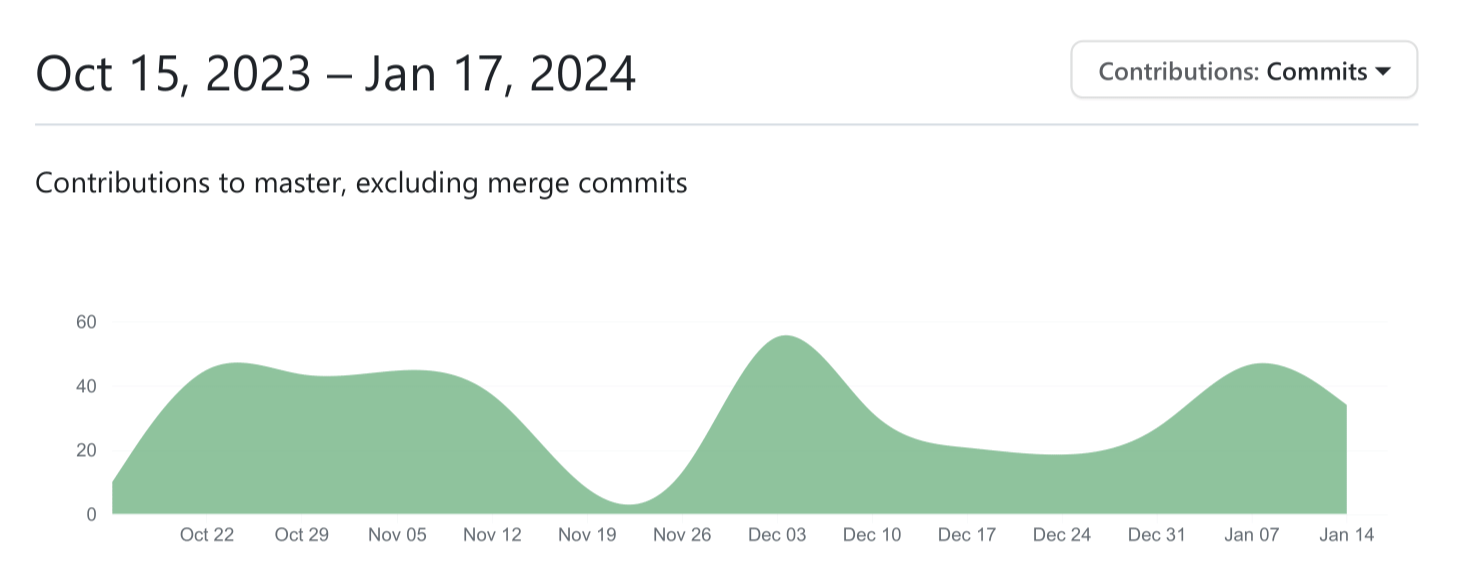
\includegraphics[width=\textwidth]{slike/promjene.png}
		\end{figure}
		
		\begin{figure}[H]
			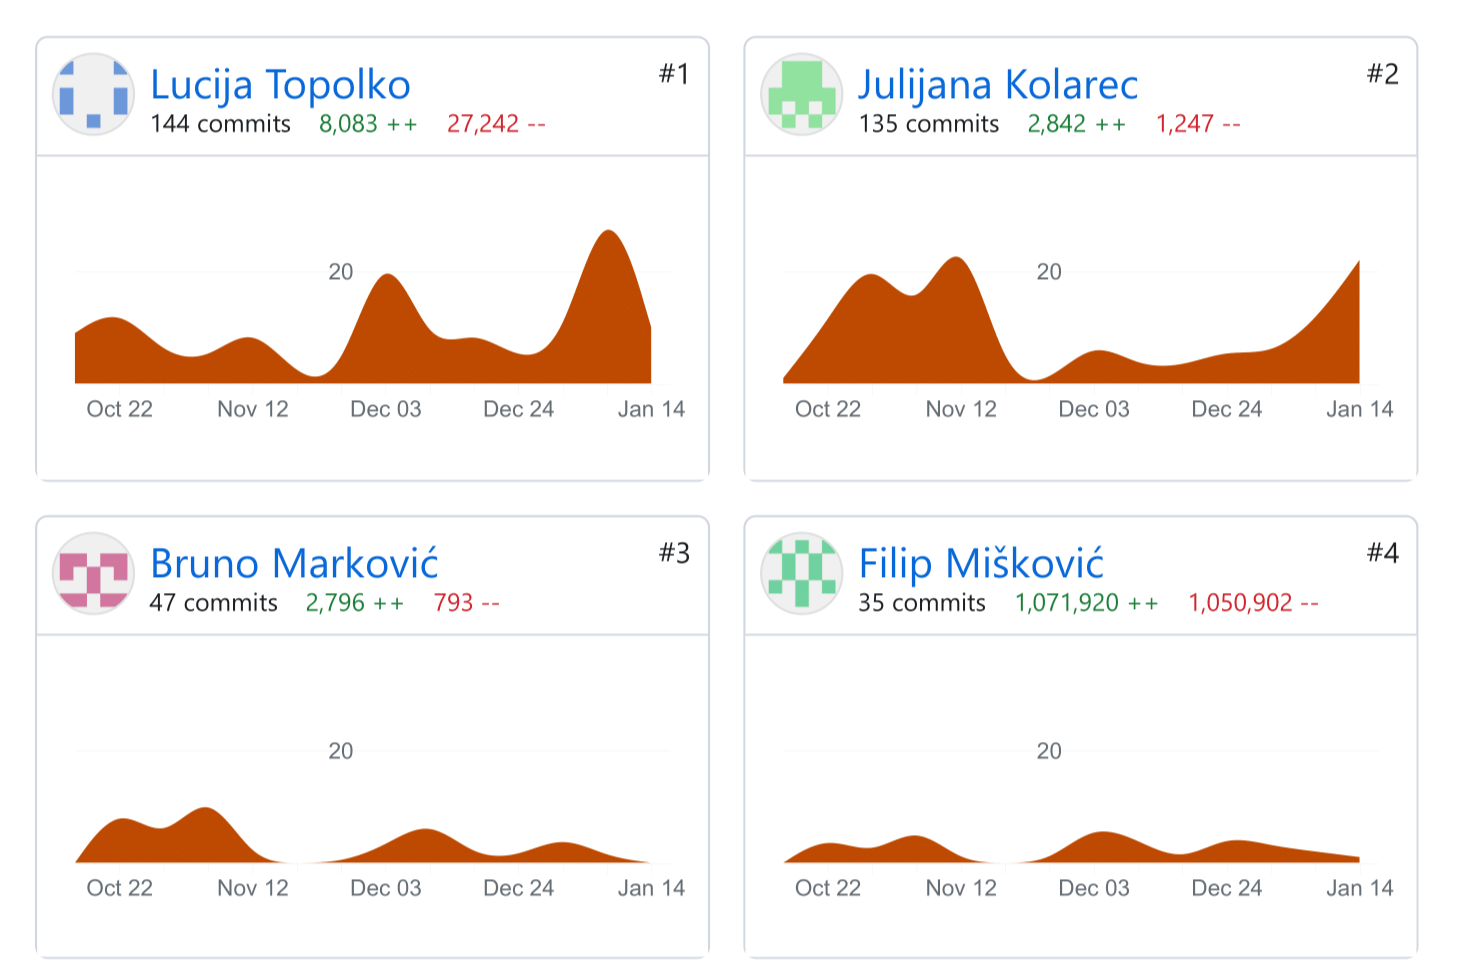
\includegraphics[width=\textwidth]{slike/promjene1.png}
		\end{figure}
		
			\begin{figure}[H]
			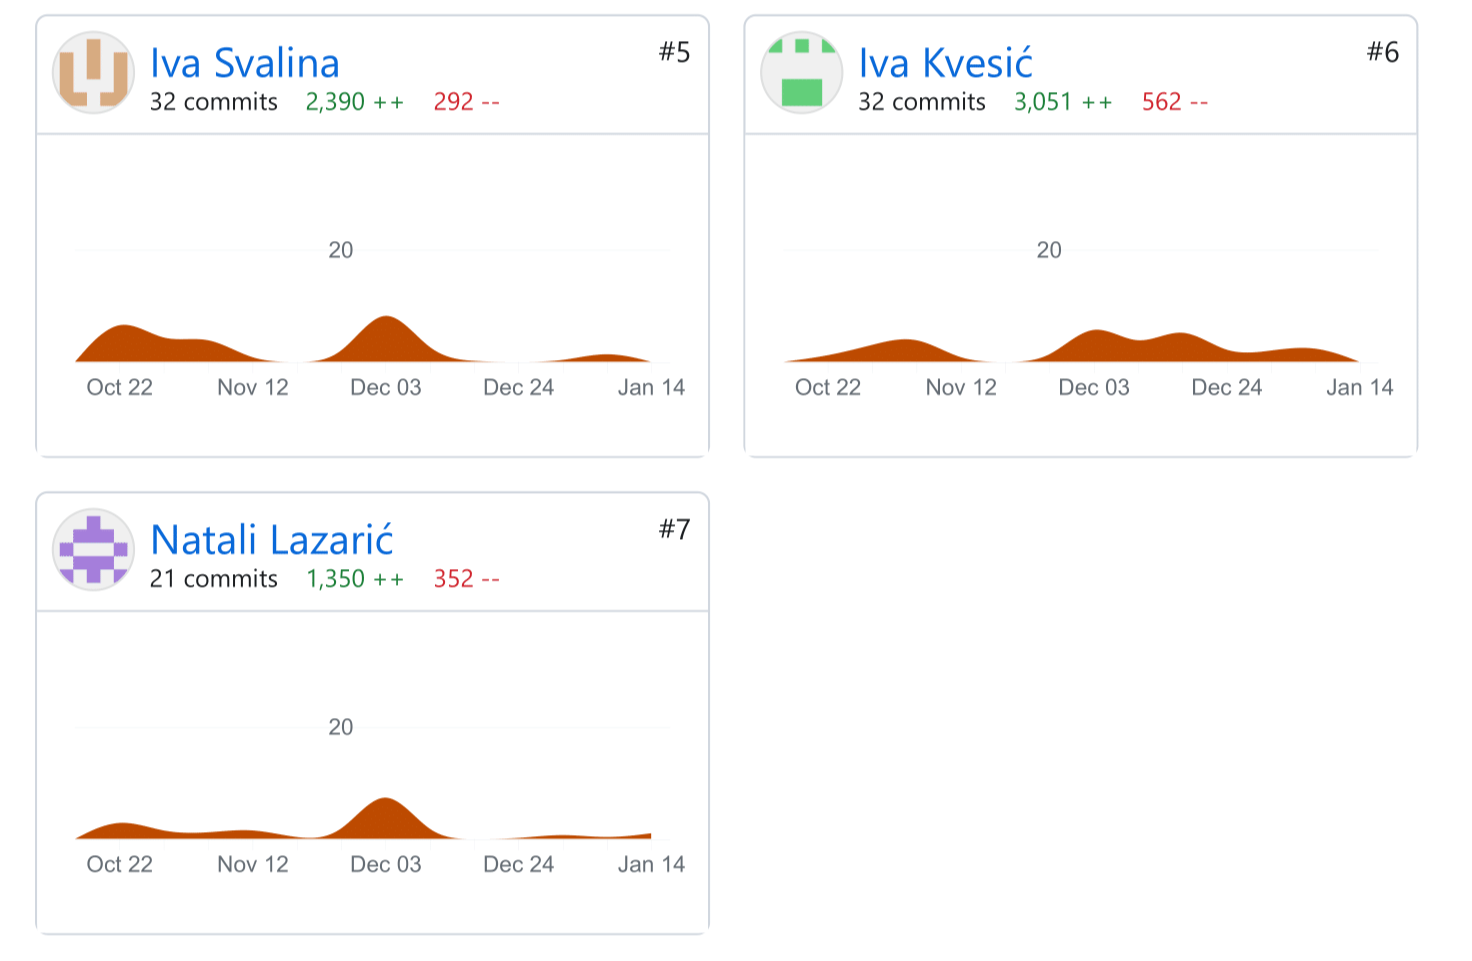
\includegraphics[width=\textwidth]{slike/promjene2.png}
			\centering
			\caption{Dijagram pregleda promjena, aktivnost na repozitoriju}
		\end{figure}
		
	